\documentclass[12pt]{article}

\usepackage{sbc-template}
\usepackage{graphicx,url}
\usepackage[utf8]{inputenc}
\usepackage[brazil]{babel}
%coisa feia
\usepackage{cite}
\usepackage{amsmath,amssymb,amsfonts}
\usepackage{algorithmic}
\usepackage{graphicx}
\usepackage{textcomp}
\usepackage[nolist]{acronym}
\begin{acronym}[LTE-Advanced]%\addtolength{\itemsep}{-0.5\baselineskip}
	\acro{3G}{3$^\text{rd}$~Generation}
	\acro{3GPP}{3rd Generation Partnership Project}
	\acro{4G}{4$^\text{th}$~Generation}
	\acro{5G}{5$^\text{th}$~Generation}
	\acro{BS}{Base Station}
	\acro{CBR}{Constant Bit Rate}
	\acro{CSI}{Channel State Information}
	\acro{DRA}{Dynamic Resource Assignment}
	\acro{DSM}{Delay-based Satisfaction Maximization}
	\acro{eNB}{Evolved Node B}
	\acro{EPA}{Equal Power Allocation}
	\acro{FER}{Frame Erasure Rate}
	\acro{FTP}{File Transfer Protocol}
	\acro{GBR}{Guaranteed Bit Rate}
	\acro{HOL}{Head Of Line}
	\acro{LTE}{Long Term Evolution}
	\acro{MOS}{Mean Opinion Score}
	\acro{NRT}{Non-Real Time}
	\acro{OFDMA}{Orthogonal Frequency Division Multiple Access}
	\acro{OFDM}{Orthogonal Frequency Division Multiplexing}
	\acro{PF}{Proportional Fair}
	\acro{QoE}{Quality of Experience}
	\acro{QoS}{Quality of Service}
	\acro{RB}{Resource Block}
	\acro{RRA}{Radio Resource Allocation}
	\acro{RRM}{Radio Resource Management}
	\acro{RT}{Real Time}
	\acro{SINR}{Signal to Interference-plus-Noise Ratio}
	\acro{SNR}{Signal to Noise Ratio}
	\acro{SISO}{Single Input Single Output}
	\acro{TTI}{Transmission Time Interval}
	\acro{TSM}{Throughput-based Satisfaction Maximization}
	\acro{UE}{User Equipment}
	\acro{VoIP}{Voice over IP}
\end{acronym}

\newcommand{\FigRef}[1]{Figure~\ref{#1}}
\newcommand{\TabRef}[1]{Table~\ref{#1}}
\newcommand{\SecRef}[1]{Section~\ref{#1}}
\newcommand{\EqRef}[1]{Equation~\ref{#1}}
\newcommand{\AppRef}[1]{Appendix~\ref{#1}}

\usepackage{graphicx}
\usepackage{caption}
\usepackage[caption=false]{subfig}

\usepackage[flushleft]{threeparttable}
\usepackage{multirow}
\usepackage{booktabs}
% SI units
\usepackage{siunitx} % provides command \SI{}{} to replace \unit{}{}
\sisetup{%
	per-mode=symbol,
}
%coisa feia     
\sloppy

\title{Utility-Based Resource Allocation Framework for QoE/QoS Maximization in OFDMA Networks}

\author{Bruno R. S. Silva\inst{1}, Pedro L. F. Lima\inst{1}, Emanuel B. Rodrigues\inst{2}, Roberto P. Antonioli \\ \inst{2} Diego A. Sousa\inst{2} Tarcsio F. Maciel\inst{2}
F. Rodrigo P. Cavalcanti\inst{2} }


\address{ Universidade Federal do Ceará
  (UFC)\\
  Caixa Postal 6.001 -- 60.455-760 -- Fortaleza -- CE -- Brasil
\nextinstitute
  Grupo de Pesquisa em Telecomunicações sem Fio (GTEL)\\
  Fortaleza, Brasil.	
  \email{\{riccelli,pedrolfalc\}@alu.ufc.br}
  \vspace{-0.4cm}
  \email{\{emanuel,roberto,diego,tarcisio,rodrigo\}@gtel.ufc.br}
}
\begin{document} 

\maketitle

\begin{abstract}
  This meta-paper describes the style to be used in articles and short papers
  for SBC conferences. For papers in English, you should add just an abstract
  while for the papers in Portuguese, we also ask for an abstract in
  Portuguese (``resumo''). In both cases, abstracts should not have more than
  10 lines and must be in the first page of the paper.
\end{abstract}
     
\begin{resumo} 
  Este meta-artigo descreve o estilo a ser usado na confecção de artigos e
  resumos de artigos para publicação nos anais das conferências organizadas
  pela SBC. É solicitada a escrita de resumo e abstract apenas para os artigos
  escritos em português. Artigos em inglês deverão apresentar apenas abstract.
  Nos dois casos, o autor deve tomar cuidado para que o resumo (e o abstract)
  não ultrapassem 10 linhas cada, sendo que ambos devem estar na primeira
  página do artigo.
\end{resumo}

\section{Introduction}
In recent years, it is noticeable the growing of users in cellular networks, which poses a challenge for the network operators to satisfy the \ac{QoS} requirements of all these users. \ac{RRA} techniques are used, for example, to provide an efficient distribution of network resources in order to improve overall system capacity. Another concept, that evaluates the users by your perception, is the \ac{QoE}, where a \ac{MOS} is given ranging between 1 to 5 \cite{ITU1996}. 
Several algorithms based on \ac{QoE} scheduling can be found in literature. The work in \cite{cho2015qoe} proposed a \ac{PF} algorithm scheduler that consider the  users' \ac{QoE} maximization and users' fairness. In \cite{mushtaq2014qoe}, a downlink scheduling method is proposed, named QoE Scheme, for improving the \ac{QoE} for \ac{VoIP} traffic in \ac{LTE} networks, in order to achieve higher user satisfaction. In \cite{liu2012novel}, the authors proposed a \ac{QoE}-based carrier scheduling scheme for multiple services that aims at maximizing the users' \ac{QoE} and showed that their approach provided some improvements in terms of QoE and fairness. The work in \cite{toseef2011user} presented a \ac{QoE}-based \ac{RRA} framework to be applied in heterogeneous wireless networks with different classes of services, such as \ac{VoIP}, \ac{FTP} and video streaming. 

In this work, we are interested at studying the benefits of considering both the \ac{QoS} and \ac{QoE} of users in resource allocation process. We propose to extend the utility-based \ac{RRA} framework and algorithms (\ac{TSM} and \ac{DSM}) presented in \cite{Rodrigues2014_Wiley} in order to consider \ac{QoE} effects in system and to maximize the users' satisfaction based on their \ac{QoE} metrics.

%Based on the work presented in \cite{Rodrigues2014_Wiley}, we propose a utility-based \ac{RRA} framework and a change in two algorithms (\ac{TSM} and \ac{DSM}) in order to consider \ac{QoE} effects in system and to maximize the users' satisfaction based on their \ac{QoE} metrics.

This work is organized as follows. Section \ref{Sec:SystemModeling} presents the system modeling considered in this work. In \SecRef{Sec:UtilFramework}, we describe the proposed utility-based \ac{RRA} framework suitable for both \ac{NRT} and \ac{RT} services. In \SecRef{sec:Performance} we show the algorithms simulated for comparison with our proposed one. Simulation assumptions are shown in \SecRef{Sec:SimulParams} and simulation results in \SecRef{Sec:Results}, while the conclusion is drawn in \SecRef{Sec:conclusion}.

\section{System Modeling}
\label{Sec:SystemModeling}
We consider a single-cell system based on \ac{OFDMA}, where the set of all \ac{UE} is indicated by $\mathcal{J} = \{1, 2, \cdots, J\}$ and all \ac{RB} to be assigned to the users are organized in a set $\mathcal{K} = \{1, 2, \cdots, K\}$.
We assume a downlink \ac{SISO} channel and consider frequency-selective Rayleigh fading where each \ac{RB} experiences flat fading. Furthermore, in our model, several independent snapshots with different user distributions are simulated, in order to capture the system performance in different coverage situations.
%

%The downlink transmission scheme is based on \ac{OFDM} using a normal prefix length and considering 14 \ac{OFDMA} symbols per \ac{TTI}. The total subcarrier bandwidth is 15 kHz, which accounts for both data and pilot symbols.
%
%A RB, which is the minimum resource block considered in the simulation, is a time-frequency chunk composed by two slots of 0.5~ms, composing the \ac{TTI} of 1~ms, and by 12 sub-carriers, which give a total bandwidth of 180kHz. It is assumed that the total power $P_t$ of the \ac{BS} is equally distributed among all \ac{RB}s. Consequently, the power $p_{k}$ allocated to \ac{RB} $k$ by \ac{BS} is $p_{k} $ = $\dfrac{P_t}{k}$.

In \ac{LTE} downlink networks, it is impossible for the \ac{CSI} to perfectly reflect the actual channel conditions at the instant of transmission due to many real-world aspects of the system implementation. In order to model part of such imperfections, we consider that the channel information $ \hat{h}_{j,k} $ sent by \ac{UE} $j$ in \ac{RB} $k$ to the \ac{eNB}, $h_{j,k}$, corresponds to the real channel measure delayed by $\Delta t$ \ac{TTI}, i.e.,
%
\begin{equation}
\hat{h}_{j,k}[n] = h_{j,k}[n -\Delta t].
\end{equation}

%From the \ac{CSI}, the instantaneous \ac{SNR} $\gamma_{j, k}$ of \ac{UE} $j$ in \ac{RB} $k$ at \ac{TTI} $n$ is given by
%%
%\begin{equation}
%\gamma_{j,k} = \dfrac{p_{k} \vert \hat{h}_{j,k} \vert^2}{\sigma^{2}},
%\end{equation}
%%
%where $\hat{h}_{j,k}$ is the channel response for the link between the \ac{BS} and the user $ j $ on \ac{RB} $k$, and $\sigma^2$ denotes the thermal noise power, which is considered constant for all \ac{UE}. The \ac{TTI} index $n$ is intentionally omitted for simplicity of notation.

Furthermore, we consider simulation scenarios comprised of one of the two following services: \ac{CBR}, which is an \ac{NRT} service; and \ac{VoIP} that is a \ac{RT} service. In order to investigate the performance of the studied \ac{RRA} techniques over the traffic models, some metrics are implemented in the simulator. In terms of satisfaction, the algorithms are evaluated considering the percentage of satisfied users given by
%
\begin{equation}
\label{Eq:Satisfaction}
\Upsilon[n] = \dfrac{J^{\text{sat}} [n]}{J},
\end{equation}
%
where $J^{\text{sat}} [n]$ is the number of satisfied users in the cell served by \ac{BS} at \ac{TTI} $n$, and $J$ is the total number of users served by \ac{BS}. Users are deemed satisfied if their \ac{MOS} at the end of their sessions are equal or higher than a threshold $(MOS_j \geq MOS_{\text{req}})$, where the session time relies on the duration of each independent simulation.
In terms of fairness, we use the Jain's fairness index, which is a measure originally proposed by \cite{JainTR-3011984} to evaluate how fair is the allocation of resources among users.

\section{Utility-Based QoE/QoS Optimization Framework}	
\label{Sec:UtilFramework}		

In this section, we present the general optimization problem of the proposed framework in \SecRef{Sec:GeneralForm}. In \SecRef{Sec:maxUtil}, the logistic function formulation is demonstrated. The specific formulations for \ac{NRT} and \ac{RT} services are shown in Sections \ref{Sec:FormNRT} and \ref{Sec:FormRT}, respectively. The resource allocation technique of our framework is shown in \SecRef{Sec:resource}.

\subsection{General Formulation}
\label{Sec:GeneralForm}

The considered optimization problem for \ac{NRT}/\ac{RT} services is the maximization of total utility with respect to the users' MOS:
\begin{subequations}\label{Eq:UtilOptProb}
	\begin{align}
	&\underset{\mathcal{K}_j}{\text{max}} \sum_{j=1}^{J} U\left(\Phi(x_j)\right), \label{Eq:UtilityOptimization}\\
	\text{subject to} \quad 
	&\bigcup_{j=1}^{J} \mathcal{K}_j \subseteq \mathcal{K}, \label{Eq:UtilityOptimizationSub1}\\ 
	&\mathcal{K}_{i} \bigcap \mathcal{K}_j = \emptyset, \quad i \neq j,  \forall i,j \in \{1,2, \ldots, J\},\label{Eq:UtilityOptimizationSub2}
	\end{align}
\end{subequations}
%
where $U(\Phi(x_j))$ is a utility function where the input parameter is the \ac{MOS} function $\Phi(x_j)$ based on a generic QoS-based variable $x_j$, $\mathcal{K}$ is the total number of resources in the system to be assigned to the users, $\mathcal{K}_j$ is the subset of resources assigned to user $j$. Constraints (\ref{Eq:UtilityOptimizationSub2}) and (\ref{Eq:UtilityOptimizationSub1}) state that the union of all subsets of resources assigned to different users must be limited to the total set of resources available in the system and that the same resource cannot be shared by two or more users in the same \ac{TTI}, respectively. 

In general, the optimum solution for the optimization problem in \EqRef{Eq:UtilOptProb} is very difficult to be obtained. A sub-optimum solution relies on splitting the problem into two stages: first, dynamic resource assignment with fixed power allocation, and second, adaptive power allocation with fixed resource assignment \cite{Gross2006}. However, it has been shown for \ac{OFDMA} systems that equal power allocation provides almost the same gains in comparison with adaptive power allocation with much lower complexity \cite{Andrews2001}. Therefore, we consider the simplified optimization problem \eqref{Eq:UtilOptProb}, which can be solved by a suitable dynamic resource assignment
with equal power allocation among the resources. 

In this framework we are interested in formulating techniques suitable for either \ac{NRT} or \ac{RT} services. Thus, we consider the variable $x_j$ to be either throughput or end-to-end packet delay, which are \ac{QoS} metrics suitable for \ac{NRT} and \ac{RT} services, respectively. In a generalized notation, we can simplify the objective function \eqref{Eq:UtilityOptimization} to become
%
\begin{equation}
\label{Eq:SimplifiedProblem}
\underset{\mathcal{K}_j}{\text{max}}\sum_{j=1}^{J} U'\left(\Phi(x_j)\right)\cdot \Phi'(x_j) \cdot \mathcal{R}_j[n],
\end{equation}
where $\mathcal{R}_j[n]$ is the instantaneous data rate of user $j$ and $U'\left(\Phi(x_j)\right)$ is the derivative of the utility function with respect to a generic \ac{MOS} function $\Phi(x_j)$  that depends on $x_j$, and  $\Phi'(x_j)$ is the derivative of the \ac{MOS} function $\Phi(x_j)$ with respect to $ x_j $. Notice that the framework  for \ac{NRT} and \ac{RT} services is aware of \ac{MOS} functions. The problem \eqref{Eq:SimplifiedProblem}  characterizes a weighted sum rate maximization, whose weights are given by
\begin{equation}
\label{Eq:GeneralWeightQoE}
wQoE_{j}^\text{NRT/RT} = U'(\Phi(x_j)),
\end{equation} 
and 
\begin{equation}
\label{Eq:GeneralWeightQoS}	
wQoS_{j}^\text{NRT/RT} = \Phi'(x_j).
\end{equation} 

On one hand, we consider that the weight given by \eqref{Eq:GeneralWeightQoE} is related to QoE because the derivative is calculated with respect to a \ac{QoE} metric (\ac{MOS} function $\Phi(x_j)$). On the other hand, we consider that the weight given by \eqref{Eq:GeneralWeightQoS} is related to \ac{QoS} because the derivative is calculated with respect to a \ac{QoS} metric (\ac{QoS} variable $x_j$). These utility-based weights assume an important role in the framework proposed in the following.

\subsection{Satisfaction Maximization Using the Logistic Utility Function}
\label{Sec:maxUtil}

In \cite{Rodrigues2014_Wiley}, the authors presented a sigmoid utility function based on a generic \ac{QoS} metric $x_j$ that was used in two techniques: Throughput-based Satisfaction Maximization \ac{TSM} and Delay-based Satisfaction Maximization \ac{DSM}. Both techniques achieve high levels of user satisfaction for \ac{NRT} and \ac{RT} services compared to classical algorithms in the \ac{4G} systems. In order to maximize user satisfaction levels, we propose the same use of the logistic utility function based on a generic \ac{QoE} metric $\Phi(x_j)$, as indicated below:
%	
\begin{equation}
U\left(\Phi(x_j)\right) = \dfrac{1}{1 + e^{\mu (\Phi(x_j) - \Phi^{\mathrm{req}}) / \sigma}},
\label{Eq:TSMQoESigmoid}
\end{equation}
%
where:
\begin{itemize} 
	\item $\mu$ is a constant (-1 or 1) that determines if the logistic function is increasing or decreasing, respectively;
	\item $\sigma$ is a non-negative parameter that determines the slope of the function; 
	\item $\Phi^{\text{req}}$ is the \ac{QoE} requirement of a given service and determines the abscissa shift of the function. It can assume values in the \ac{MOS} range.
\end{itemize}

The marginal utility function has a bell-shaped format and is given by
%
\begin{equation}
\label{Eq:wQoE}
U'\left(\Phi\left(x_j\right)\right)=\dfrac{- \mu  e^{\mu (\Phi(x_{j}[n]) - \Phi^{\text{req}}) / \sigma}}{\sigma (1 + e^{\mu (\Phi(x_{j}[n]) - \Phi^{\text{req}}) / \sigma})^{2}}.
\end{equation}

Notice that the higher is the value of the parameter $\sigma$, the steeper is the sigmoid. A function of $ \Phi^{\mathrm{req}}$ was developed to obtain $\sigma$ so that a desired step-shaped logistic function can be achieved, where the utility is equal to a value $\delta$ when the QoE metric achieves a proportion $\rho$ of the QoE requirement $\Phi^{\text{req}}$. Thus, we have
%
\begin{equation}
\label{Eq:Sigma}
\sigma = \dfrac{\mu \cdot (\rho - 1) \cdot \Phi^{\text{req}}}{\log \Big( \dfrac{1}{\delta} - 1\Big)}.
\end{equation}

The algorithms proposed in this work use only an increasing logistic function that is obtained when the $\mu$ parameter is set to -1 for both services, as presented in \FigRef{Fig:UserUtility}. This is a novelty compared to the work in \cite{Rodrigues2014_Wiley}, which proposes algorithms based on throughput and delay that use increasing ($\mu$ = -1) and decreasing ($\mu$ = 1) sigmoidal utility functions for \ac{NRT} and \ac{RT} services, respectively.

\begin{figure}
	\centering
	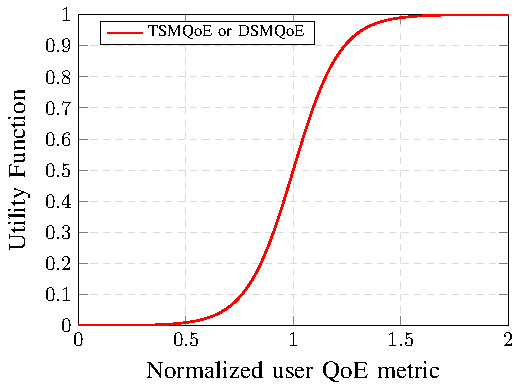
\includegraphics[width=0.55\linewidth]{figs_wp2/figs_BRUNO_PEDRO/userUtility}
	\caption{NRT/RT utility function}	
	\label{Fig:UserUtility}
\end{figure}	

The narrow shaped utility function   means that a user rapidly becomes satisfied if its \ac{QoE} metric (\ac{MOS}) approaches or exceeds the requirement. On the opposite, users become unsatisfied when their \ac{MOS} is below the requirement. Satisfactory results  were obtained when $ \delta = 0.01$, $\rho = 0.50$ and $\Phi^{\text{req}} = 1$. For these values we obtain from \EqRef{Eq:Sigma} $\sigma = 0.1088$. \FigRef{Fig:Bell} shows the bell shaped marginal utility function, which is the derivative of the sigmoidal utility function of \FigRef{Fig:UserUtility}. 	

\begin{figure}
	\centering
	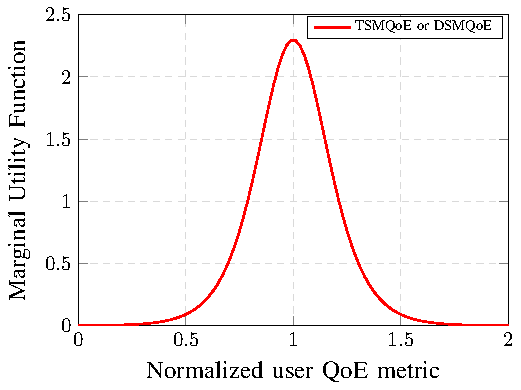
\includegraphics[width=0.55\linewidth]{figs_wp2/figs_BRUNO_PEDRO/sino}
	\caption{NRT/RT marginal utility function}	
	\label{Fig:Bell}	
\end{figure}

%A normalization by the \ac{QoE} requirement $\Phi^{\mathrm{req}}$ is considered in this work, i.e., $\Phi(x_j)/\Phi^{\mathrm{req}}$  and therefore the value $ \Phi^{\mathrm{req}}$ previously described is $ \Phi^{\mathrm{req}} = 1$. This explains the reason behind the normalized user QoE metric in the abscissa axises of figures \ref{Fig:UserUtility} and \ref{Fig:Bell}. By performing this normalization, the proposed framework can operate independently of the considered \ac{QoE} requirement $\Phi^{\mathrm{req}}$.

\subsection{Formulation for NRT Services}
\label{Sec:FormNRT}
%
\subsubsection{Throughput Calculation}
\label{Sec:THRU}
The \ac{NRT} formulation uses as primary metric the throughput, which is calculated using a exponential filter \cite{UFC40_WP2_TR_02_JSM}. As such, the throughput of user $j$ is

\begin{equation}
\label{Eq:ThroughputCalculation}
T_{j}\left[n\right] = \left(1 - f_{\mathrm{thru}}\right) \cdot T_{j}\left[n-1\right] + f_{\mathrm{thru}} \cdot \mathcal{R}_j[n],
\end{equation}

where $\mathcal{R}_j[n]$ is the instantaneous data rate of user $j$ and $f_{\mathrm{thru}}$ is a filtering constant.

\subsubsection{QoE Mapping Function}
Note that the original framework proposed in \cite{Rodrigues2014_Wiley} is based on \ac{QoS}. In order to extend it and consider \ac{QoE}, it is necessary to use a mapping function and map throughput values into opinion scores. Therefore, we use a \ac{MOS} function $\Phi(T_j [n])$ described in \cite{Poncela2014}, which is shown in \EqRef{MOS_FUNC_NRT} and \FigRef{Fig:MOSTSMQoE}. The expression or the mapping function is:
% 
\begin{equation}\label{MOS_FUNC_NRT}
\Phi\left(T_j[n]\right)= 5 - \frac{578}{1+\left(\dfrac{T_j[n] + 541.1}{45.98}\right)^{2}}.        
\end{equation}

\begin{figure}
	\centering
	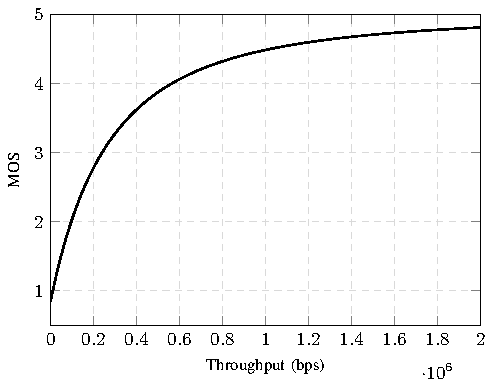
\includegraphics[width=0.55\linewidth]{figs_wp2/figs_BRUNO_PEDRO/MOSTSMQoE}
	\caption{MOS mapping function for NRT services}
	\label{Fig:MOSTSMQoE}
\end{figure}
%%CUTTING
%
%\subsubsection{Utility-Based Weights Calculation}
%
%As explained in \SecRef{Sec:GeneralForm}, our optimization problem depends on two weights, $wQoS$ and $wQoE$.
%It can be seen in details in \AppRef{AppendixA}, how the weight $wQoE^{\text{NRT}}$ can be calculated for \ac{NRT} services. Its expression is given by:
%
%\begin{equation}
%\label{wQoERT}
%\begin{split}    
%wQoE_{j}^{\text{NRT}} &= \dfrac{\partial U\left(\Phi\left(T_j[n]\right)\right)}{\partial \Phi} \\&= \dfrac{\partial }{\partial \Phi}  \left(\dfrac{1}{1 + e^{\mu (\Phi(T_{j}[n]) - \Phi^{\text{req}}) / \sigma}}\right)\\
%&= \dfrac{- \mu  e^{\mu (\Phi(T_{j}[n]) - \Phi^{\text{req}}) / \sigma}}{\sigma \left(1 + e^{\mu (\Phi(T_{j}[n]) - \Phi^{\text{req}}) / \sigma}\right)^{2}}.
%\end{split}
%\end{equation}
%
%Notice that \EqRef{wQoERT} is equal to \EqRef{Eq:wQoE}, where $\Phi(x_j) = \Phi(T_j[n])$. Moreover, according to  \AppRef{AppendixA}, $wQoS_{j}^{\text{NRT}}$ can be calculated by:
%%
%\begin{equation}
%\label{Eq:wQoS_TSMQoE}
%wQoS_{j}^{\text{NRT}} = \dfrac{\partial \Phi\left(T_j[n]\right)}{\partial T_{j}} =  \frac{0.5468 \cdot \left(T_j[n]+541.1\right)}{ \left[1+\left(\dfrac{T_j[n] + 541.1}{45.98}\right)^{2}\right]^{2}}.
%\end{equation}
%
%The considered objective function of the optimization problem for \ac{NRT} services is given by:
%%         
%\begin{equation}
%\underset{\mathcal{K}_j}{\text{max}} \sum_{j=1}^{J} U\left(\Phi\left(T_j[n]\right)\right). \label{Eq:Util_Opt_JointNRT}        
%\end{equation}
%
%As commented in \SecRef{Sec:GeneralForm} and demonstrated in \AppRef{AppendixA}, the original problem \ref{Eq:Util_Opt_JointNRT}:
%%
%\begin{equation}    \label{Eq:modifiedNRTproblem}
%\underset{\mathcal{K}_j}{\text{max}} \sum_{j=1}^{J} \dfrac{\partial U\left(\Phi\left(T_j[n]\right)\right)}{\partial \Phi} \cdot \dfrac{\partial \Phi\left(T_j[n]\right)}{\partial {T_j}} \cdot \mathcal{R}_j\left[n\right].
%\end{equation}

\subsection{Formulation for RT Services}
\label{Sec:FormRT}

\subsubsection{End-to-End Delay Estimation}
In this section we show how the end-to-end delay is used in this work. As described in \SecRef{Sec:SystemModeling}
we simulate the downlink of an LTE network. Thus, the end-to-end packet delay is calculated by the sum of the \ac{HOL} packet delay imposed by the radio access network ($d_j ^{\text hol}$) and the packet delay imposed by the Core Network ($d_j^{\text core}$):
%
\begin{equation}
\label{Eq:endToEndDelay}
d_j[n] = d_{j}^\text{hol}[n] + d_j^\text{core}[n].
\end{equation}

We use a recursive model to calculate the \ac{HOL} packet delay as follows \cite{Rodrigues2014_Wiley}:
%
\begin{equation}
\label{Eq:HOL_Delay}
d_{j}^\mathrm{hol}\left[n+1\right] = d_{j}^\mathrm{hol}\left[n\right] + t_{\text{tti}} - \frac{1}{L} \cdot \left( \frac{\mathcal{R}_{j}[n] \cdot t_{\text{tti}}}{S_\mathrm{p}}\right),
\end{equation}
%
where $t_{\text{tti}}$ is the duration of the \ac{TTI} in seconds, $L$ is the packet arrival rate, $S_\mathrm{p}$ is the packet size, and $\mathcal{R}_{j}[n]$ is the instantaneous achievable transmission rate on \ac{TTI} $n$.

We model the core network delay $d_j^\text{core}$ following a truncated Gaussian distribution with mean fixed at \SI{105}{\ms} and using the $3\sigma$ rule to generate random values from 0 to \SI{210}{\ms}, as shown in \FigRef{Fig:EndToEndDelay}. %
Thus, $d_j^\text{core} = \max(0; \min(0.210; d(\mu, \sigma)))$, where $ d(\mu, \sigma) $ follows a Gaussian distribution with mean $ \mu $ and standard deviation $ \sigma $. %
This model aims to increase the variability in system simulations. The work in \cite{liu2012novel}, which uses the same MOS and simulation scenario, consider the core network delay as a fixed value of 100 ms. 

\begin{figure}
	\centering
	\includegraphics[width=0.55\linewidth,page=5]{figs_wp2/figs_BRUNO_PEDRO/plots}
	%	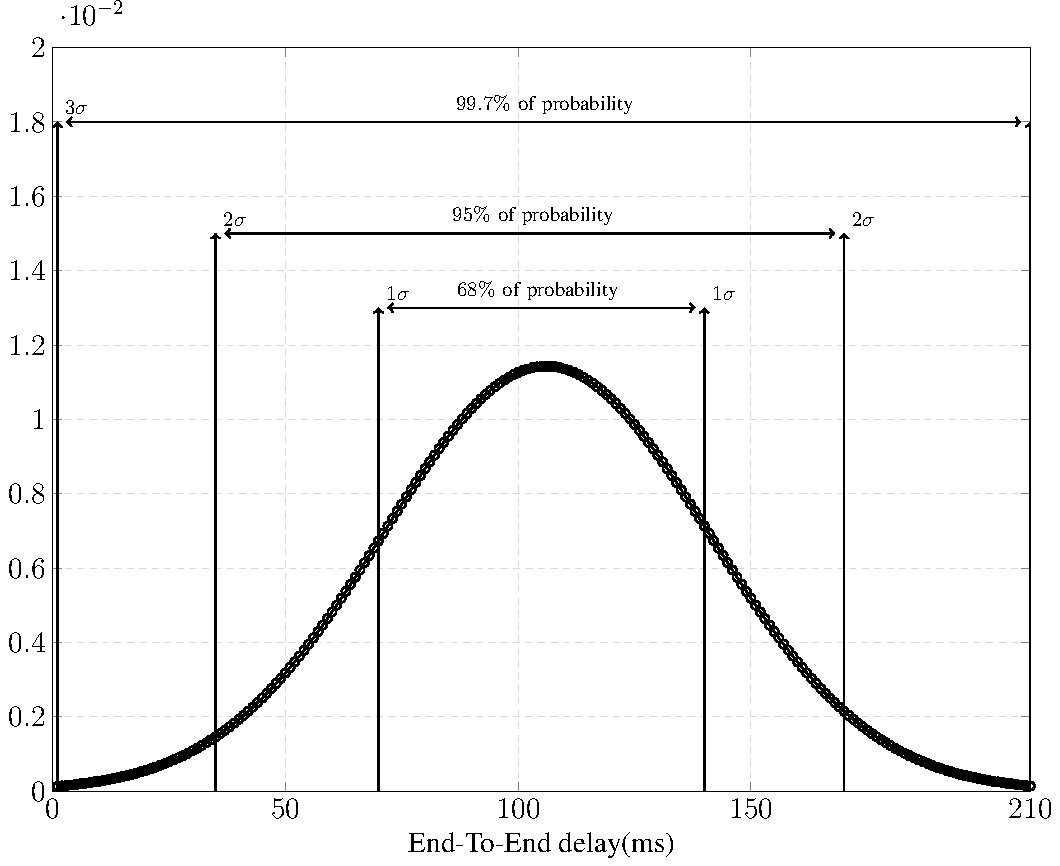
\includegraphics[width=0.55\linewidth]{figs_wp2/figs_BRUNO_PEDRO/EndToEndDelay}
	\caption{Core Network delay model.}
	\label{Fig:EndToEndDelay}
\end{figure}	

\subsubsection{E-Model}
The $ R $ factor is the primary output of the ITU-T E-model G.107 \cite{itu2005107} calculations. It is a scalar ranging between 0 and 100 that provides a prediction of the expected voice service quality which is mapped to a \ac{MOS} value in our formulation. The $ R $ factor is given by
%
\begin{equation}
\label{GeneralRFactor}
R = R_o - I_s - I_d - I_e + A,
\end{equation} 
%
where $R_o$ is the basic signal-to-noise ratio, $I_s$ is a combination of all impairments which occur almost simultaneously within the voice signal, $I_d $ represents the impairments caused by delay, $I_e$ represents the impairments caused by codecs and random packet losses, and the advantage factor $A$ allows for a compensation of impairment factors in the modeling. According to \cite{itu2005107} and \cite{cole2001voice}, this value is equal to 10.
For simplicity, \cite{cole2001voice} proposes an equivalent estimation of the $ R $ factor according to the G.729a codec:
%
\begin{align}
R\left(d_j[n]\right) \approx 94.2 - 0.024 \cdot d_j[n] - 0.11 \cdot \left(d_j[n] - 177.3\right) \cdot  \notag \\ H\left(d_j[n] - 177.3\right) - 11 - 40 \cdot \ln\left(1 + 10\cdot \varepsilon\right) + 10. &	
\end{align}
%
where $H(x)$ is the unit step function and $\varepsilon$ is the network error probability. Notice that $I_e$ in \EqRef{GeneralRFactor} was estimated in \cite{cole2001voice} under random packet loss conditions.
%		
%\begin{figure}
%	\centering
%	\includegraphics[width=0.55\linewidth,page=8]{figs_wp2/figs_BRUNO_PEDRO/plotsCSI}
%	\caption{$ R $ factor to \ac{RT} services considering different Core Network errors.}
%	\label{Fig:RxNetworkError}
%\end{figure}
%		

\subsubsection{QoE Mapping Function}	

The  \ac{MOS} function $\Phi\left(R\left(d_j[n]\right)\right)$ for the voice service proposed in \cite{cole2001voice} is illustrated  in \FigRef{Fig:MOSxNetworkError} considering different values of the core network error and it is expressed below as: 
\begin{multline}\label{MOS_DELAY_FUNC}
\Phi\left(R\left(d_j[n]\right)\right) = 1+ 0.035\cdot R\left(d_j[n]\right)+ R\left(d_j[n]\right)\cdot \\
\left(R\left(d_j[n]\right) - 60\right) \cdot \left(100 - R\left(d_j[n]\right)\right)\cdot 7 \cdot  10^{-6}.
\end{multline}

\begin{figure}
	\centering
	\includegraphics[width=0.55\linewidth,page=7]{figs_wp2/figs_BRUNO_PEDRO/plotsCSI}
	\caption{MOS mapping function for RT services considering different core network errors.}
	\label{Fig:MOSxNetworkError}		
\end{figure}

%\subsubsection {Utility-Based Weights Calculation}
%Regarding Equations (\ref{Eq:GeneralWeightQoE}) and (\ref{Eq:wQoE}) in \SecRef{Sec:UtilFramework}, $wQoE_{j}^{\text{RT}}$ can be calculated by:
%%
%\begin{equation}
%\label{wQoE}
%\begin{split}	
%wQoE_{j}^{\text{RT}} &= \dfrac{\partial U\left(\Phi\left(R\left(d_j[n]\right)\right)\right)}{\partial \Phi} \\&= \dfrac{\partial }{\partial \Phi}  	\left(\dfrac{1}{1 + e^{\mu (\Phi(R(d_j[n])) - \Phi^{\text{req}}) / \sigma}}\right)	\\&= \dfrac{- \mu  e^{\mu (\Phi(R(d_j[n])) - \Phi^{\text{req}}) / \sigma}}{\sigma \left(1 + e^{\mu (\Phi(R(d_j[n])) - \Phi^{\text{req}}) / \sigma}\right)^{2}}
%\end{split}
%\end{equation}
%
%Considering \EqRef{Eq:GeneralWeightQoS} in \SecRef{Sec:UtilFramework} and evaluating the MOS expression in \EqRef{MOS_DELAY_FUNC}, the QoS-based weight is calculated as:
%%
%\begin{equation}
%\label{Eq:wQoSDSMQoE}
%wQoS_{j}^{\text{RT}} = \Phi'\left(R\left(d_j[n]\right)\right) = \dfrac{\partial \Phi\left(R\left(d_j[n]\right)\right)}{\partial R} \cdot \dfrac{\partial R\left(d_j[n]\right)}{\partial d_j}, 
%\end{equation}
%%
%where, according to \AppRef{AppendixB}, 
%%
%\begin{equation}
%\dfrac{\partial \Phi\left(R\left(d_j[n]\right)\right)}{\partial R} = 0.035 + 320\cdot7 \cdot  10^{-6}R\left(d_j[n]\right), 
%\end{equation}
%%
%and
%%			
%\begin{equation}
%\dfrac{\partial R\left(d_j[n]\right)}{\partial d_j} = - 0.024 - 0.11 \cdot H\left(d_j[n] - 177.3\right) - D\left(d_j[n] - 177.3\right)\cdot \left(0.11d_j[n] - 19.503\right),
%\end{equation}
%%
%where $H(x)$ is the unit step function and $D(x)$ is the unitary impulse function. Looking at \FigRef{Fig:MOSxNetworkError}, we can see that the function $\Phi(R(d_j[n]))$ is decreasing, so its derivative with respect to to $d_j$ given by \EqRef{Eq:wQoSDSMQoE} is negative. Because of that, we use a module function to avoid a negative value in the resource allocation procedure (more details in \SecRef{Sec:resource}).
%
%The considered objective function of the optimization problem for \ac{RT} services is given by:
%%
%\begin{equation}
%\underset{\mathcal{K}_j}{\text{max}} \sum_{j=1}^{J} U\left(\Phi\left(R\left(d_j[n]\right)\right)\right), \label{Eq:Util_Opt_Joint}
%\end{equation}
%%
%where $d_j[n] $ is the end-to-end delay. As commented in \SecRef{Sec:GeneralForm} and demonstrated in \AppRef{AppendixB}, the original problem (\ref{Eq:Util_Opt_Joint}) can be simplified in the form:
%%
%\begin{equation}
%\label{Eq:modifiedRTproblem}
%\underset{\mathcal{K}_j}{\text{max}} \sum_{j=1}^{J} \left. \dfrac{\partial U\left(\Phi\left(R\left(d_j[n]\right)\right)\right)}{\partial \Phi}\right\vert_{\Phi = \Phi \left(R\left(d_{j}[n - 1]\right)\right)} \cdot \left. \dfrac{\partial \Phi\left(R\left(d_j[n]\right)\right)}{\partial {d_j}} \right\vert_{d_{j}[n] = d_{j}[n - 1]}\cdot \mathcal{R}_j\left[n\right].
%\end{equation}

\subsection{Resource Allocation}
\label{Sec:resource}
This work proposes two \ac{RRA} algorithms that consider both \ac{QoE} and \ac{QoS}. These algorithms are extensions of the \ac{TSM} and \ac{DSM} algorithms proposed in \cite{Rodrigues2014_Wiley}, and are called TSMQoE and DSMQoE, respectively.

It is worth to mention that, apart from being formulated for an \ac{LTE} network, the \ac{RRA} algorithms shown in this section can be applied to any modern cellular system.

\subsubsection{TSMQoE Algorithm for NRT Scenario}
Since the simplified optimization problem given by \EqRef{Eq:SimplifiedProblem} is a weighted sum maximization problem, we can find a closed form solution for that \cite{Art:Song2005_p2,Proc:Hosein2002}. Therefore we have that the user with index $j^\star$ is chosen to transmit on \ac{RB} $k$ in \ac{TTI} $n$ if it satisfies the condition given by
%
\begin{equation}
\label{Eq:argmaxTSMQoE}
\begin{split}
j^{\star} &= \arg\max_{j} \left\{\dfrac{\partial U\left(\Phi\left(T_j[n]\right)\right)}{\partial \Phi} \cdot \dfrac{\partial \Phi\left(T_j[n]\right)}{\partial {T_j}} \cdot r_{j,k}\left[n\right]\right\} \\&= \arg\max_{j} \left\{wQoE_{j}^{\text{NRT}}\cdot wQoS_{j}^{\text{NRT}} \cdot r_{j,k}\left[n\right]\right\},
\end{split}
\end{equation}
%	
where $r_{j,k}[n]$ denotes the instantaneous achievable transmission rate of user $ j $ with respect to \ac{RB} $k$ at \ac{TTI} $n$, $wQoE_{j}^{\text{NRT}}$ and $wQoS_{j}^{\text{NRT}}$ are the QoE- and QoS-based weights associated to user $j$ using an NRT service. A tiebreaker based in channel conditions is used if more than one user has the same priority. Notice that these utility-based weights play a crucial role in the resource allocation. 

%The combination (multiplication) of the QoE- and QoS-based weights is depicted in \FigRef{Fig:combinatedWeightsTSMQoE} and the QoS-based weight for the TSMQoS algorithm is presented in \FigRef{fig21}.

As commented in \SecRef{Sec:maxUtil} the logistic function has its input parameter and requirement normalized by the parameter $\Phi^{\mathrm{req}}$ that is equivalent for both QoS and QoE algorithms. However, due to this normalization, only the final weight for the TSMQoS algorithm is centered at the normalized requirement, while the combined weight for the TSMQoE algorithm has its peak below the normalized requirement because of the weights' multiplication. 

%\begin{figure}[htb!]
%	\centering
%	\subfloat[Combination of the QoE- and QoS-based weights used in the TSMQoE algorithm.]{
%		%		\centering
%		\includegraphics[width=0.49\textwidth, page=3]{figs_wp2/figs_BRUNO_PEDRO/plots}
%		\label{Fig:combinatedWeightsTSMQoE}
%	}		
%	\subfloat[QoS-based weight used in the TSMQoS algorithm.]{
%		\centering
%		\includegraphics[width=0.49\textwidth, page=4]{figs_wp2/figs_BRUNO_PEDRO/plots}
%		\label{fig21}
%	}
%	\caption{Weights for TSMQoE and TSMQoS algorithms considering QoE-based requirement of 4 (MOS value) and QoS-based requirement of 563.4~kbps.}
%	\label{Fig:WeightsForTSMQoE}
%\end{figure} 

\subsubsection{DSMQoE Algorithm for \ac{RT} Scenario}
Since the simplified optimization problem given by \EqRef{Eq:SimplifiedProblem} is a weighted sum maximization problem, we can find a closed form solution for that \cite{Art:Song2005_p2,Proc:Hosein2002}. Therefore, we have that the user with index $j^\star$ is chosen to transmit on \ac{RB} $k$ in \ac{TTI} $n$ if it satisfies the condition given by
%
\begin{equation}
\label{Eq:argmaxDSMQoE}
\begin{split}
j^{\star} &= \arg\max_{j} \left\{\dfrac{\partial U\left(\Phi\left(R\left(d_j[n]\right)\right)\right)}{\partial \Phi} \cdot \left| \dfrac{\partial \Phi\left(R\left(d_j[n]\right)\right)}{\partial {d_j}} \right| \cdot r_{j,k}\left[n\right]\right\}\\ &= \arg\max_{j} \left\{wQoE_{j}^{\text{RT}}\cdot |wQoS_{j}^{\text{RT}}| \cdot r_{j,k}\left[n\right]\right\}.
\end{split}
\end{equation}
%
$wQoE_{j}^{\text{RT}}$ and $wQoS_{j}^{\text{RT}}$ are the QoE- and QoS-based weights associated to user $j$ using an \ac{RT} service. A tiebreaker based in channel conditions is used if more than one user has the same priority.

%The combination (multiplication) of the QoE- and QoS-based weights is depicted in \FigRef{Fig:combinatedWeightsDsSMQoE} and the QoS-based weight for the DSMQoS algorithm is presented in \FigRef{fig2}.
%
%\begin{figure}[htb!]
%	\centering
%	\subfloat[Combination of the QoE- and QoS-based weights used in the DSMQoE algorithm.]{
%		%		\centering
%		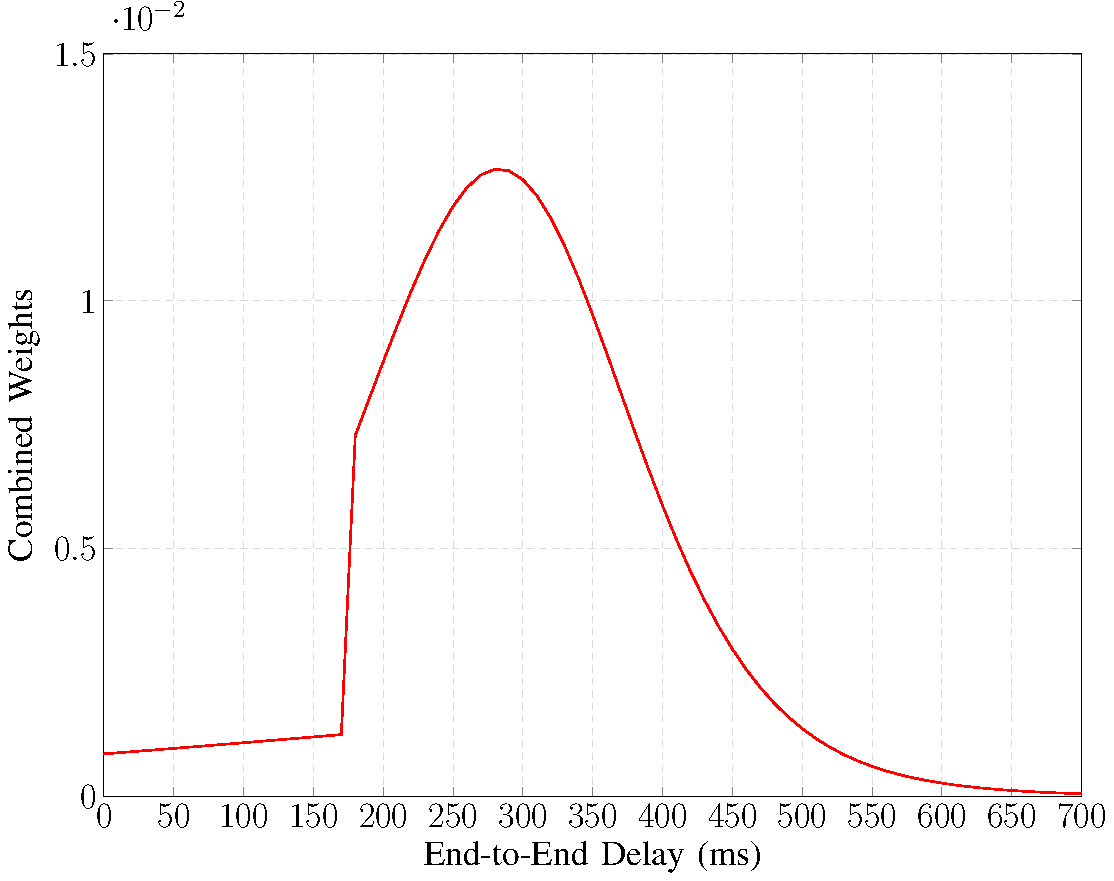
\includegraphics[width=0.49\textwidth, page=1]{figs_wp2/figs_BRUNO_PEDRO/plots}
%		\label{Fig:combinatedWeightsDsSMQoE}
%	}		
%	\subfloat[QoS-based weight used in the DSMQoS algorithm.]{
%		\centering
%		\includegraphics[width=0.49\textwidth, page=2]{figs_wp2/figs_BRUNO_PEDRO/plots}
%		\label{fig2}
%	}
%	\caption{Weights for DSMQoE and DSMQoS algorithms considering QoE-based requirement of 4 (MOS value) and QoS-based requirement of 250~ms.}
%	\label{Fig:WeightsForDSMQoE}
%\end{figure} 
\section{Performance Evaluation}
\label{sec:Performance}

This section presents the resource allocation algorithms taken from the literature that were evaluated and compared with the proposed \ac{RRA} techniques, the simulation scenario, and the obtained simulation results. In \SecRef{Sec:stateOfTheArtAlg}, the algorithms used for comparison against our proposal are presented. The parameters adopted in our simulations are described in \SecRef{Sec:SimulParams} and the obtained results are presented and discussed in \SecRef{Sec:Results}.

\subsection{State-of-The-Art Algorithms}
\label{Sec:stateOfTheArtAlg}

\subsubsection{NRT Scenario}
\label{PerfNRT}

\paragraph{Throughput-Based Satisfaction Maximization\\}
The \ac{TSM} is an RRA technique based on the Utility Theory that was proposed in \cite{Rodrigues2014_Wiley}. It uses a sigmoid function in order to maximize user satisfaction. The authors propose in \cite{Rodrigues2014_Wiley} that the user with index $j^\star$ is chosen to transmit on resource $k$ in \ac{TTI} $n$ following the condition below:
%  
\begin{equation}
\label{Eq:TSMArgmax}
j^{\star} = \underset{j}{\text{arg max}}\Big\{w_j \cdot {r_{j, k}[n]}\Big \},
\end{equation}
%
where
%
\begin{equation}
\label{TSMMarginal}
w_{j} = \dfrac{\partial U\left(T_{j}[n]\right)}{\partial T_{j}} = \dfrac{- \mu  e^{\mu \left(T_{j}[n] - T_{j}^{\text{req}}\right) / \sigma}}{\sigma \left(1 + e^{\mu (T_{j}[n] - T_{j}^{\text{req}}) / \sigma}\right)^{2}}.
\end{equation}
%
that comes from a logistic bell-shaped marginal utility function.  

\paragraph{Proportional Fairness QoE\\}
The Proportional Fairness \ac{QoE} algorithm  is a version of \ac{PF} with \ac{QoE} properties. Note that the PFQoE algorithm proposed in \cite{cho2015qoe}  uses a logarithmic utility function from the generalized PF algorithm and a MOS model based on a Bezier curve. However, we simulate this algorithm with the same MOS presented in \SecRef{Sec:FormNRT} in order to compare it with our proposed TSMQoE technique. A user with index $j^\star$ is chosen to transmit on resource $k$ in \ac{TTI} $n$ following the condition below:
%
\begin{equation}
\label{Eq:PFQoEArgmax}
j^{\star} = \underset{j}{\text{arg max}} \left\{ {\dfrac{  \Phi^{'}\left(T_j[n]\right) }{\left(\Phi\left(T_j[n]\right) - \chi\right)} \cdot r_{j, k}[n]} \right\},
\end{equation}
%
where $\Phi^{'}\left(T_j[n]\right) = \dfrac{\partial\Phi\left(T_j[n]\right)}{\partial T_j}$ is the \ac{MOS} derivative  with respect to throughput $T_j$ and $\chi$ is the minimum MOS value.  
\subsubsection{\ac{RT} Scenario}

\paragraph{Delay-Based Satisfaction Maximization\\}
The \ac{DSM} technique was firstly proposed in \cite{Rodrigues2014_Wiley}. It uses a decreasing sigmoidal utility function, which means that the higher the HOL delay, the lower the utility derived from the network. The authors in \cite{Rodrigues2014_Wiley} showed that DSM achieved higher user satisfaction levels than other algorithms found in the literature. The resource allocation performed by this algorithm states that the chosen user should be 
\begin{equation}
\label{Eq:DSMArgmax}
j^{\star} = \underset{j}{\text{arg max}}\Big\{w_j \cdot {r_{j, k}[n]}\Big \},
\end{equation}
%
where
%
\begin{equation}
\label{DSMMarginal}
w_{j} = \dfrac{\partial U(d_{j}[n])}{\partial d_{j}} = \dfrac{- \mu  e^{\mu (d_{j}[n] - d_{j}^{\text{req}}) / \sigma}}{\sigma \left(1 + e^{\mu (d_{j}[n] - d_{j}^{\text{req}}) / \sigma}\right)^{2}}
\end{equation}
%
which comes from a logistic bell-shaped marginal utility function. Notice that in $w_{j}$ the end-to-end delay $d_{j}[n]$ is considered, instead of the $d_{j}^\mathrm{hol}\left[n\right]$  as in the original DSM technique proposed in \cite{Rodrigues2014_Wiley}. This adaptation was performed in order to compare the original DSM with the DSMQoE.

\paragraph{QoE Scheme\\} 
The QoE Scheme \cite{mushtaq2014qoe} has a structure that maximizes user's \ac{MOS} beyond a fair factor. The $j^\star$ user is chosen to transmit on resource $k$ in \ac{TTI} $n$ if it satisfies the condition given by
%
\begin{equation}
\label{Eq:QoESchemeArgmax}
j^{\star} = \underset{j}{\text{arg max}}\left\{ {{\Phi\left(R\left(d_j[n]\right)\right)\cdot \nu_j\cdot \left(\frac{GBR_j}{r_{j, k}[n]}\right)^\eta}}\right\}.
\end{equation}
%
where:
%
\begin{itemize}
	\item $\Phi\left(R\left(d_j[n]\right)\right)$ is the same \ac{MOS} function that we use in this work;
	\item $\nu_j$ is a property of Proportional Fair \cite{Kelly1997} used for a fair resource distribution given by $\dfrac{r_{j, k}[n]}{T_j[n]}$;
	\item $GBR_j$ is the guaranteed bit rate requirement for the \ac{VoIP} user $j$;
	\item $\eta$ is a tunable exponential factor for $GBR$ \ac{VoIP} traffic that can be used to increase priority of the user $j$ in order to fulfill the $GBR_j$ requirement.
\end{itemize}

This algorithm was chosen for comparison because it uses the users' end-to-end (as a parameter for the MOS mapping function) in order to guarantee a minimum bit rate for the users.

\subsection{Simulation Parameters}
\label{Sec:SimulParams}
%
%Some general simulation assumptions considered in this work are listed in Table 1. %
Different services are employed to evaluate the performance of the algorithms for RT services or for NRT services. The \ac{CBR} traffic model used in this work generates packets at 563.4~kbps (corresponding to MOS of 4), where the packet size and the inter-arrival time are fixed to 4507~bits and 8~ms, respectively. Other characteristic of this application is that delayed packets are not discarded, causing an  increase in the buffer size \cite{Nasralla2013}. The \ac{VoIP} traffic model is based on an ON/OFF Markov chain with packet size of 320~bits generated every 20~ms. Moreover, delayed packets with end-to-end delay $d_j$ higher than 250~ms are discarded from the \ac{eNB} buffer. 

Furthermore, we consider imperfect \ac{CSI}, where users are able to estimate their channels properly, but the \ac{eNB} receives these values with delay $\Delta t$ varying between 0 and 40 TTIs.	  

%\begin{table}[!htb]
%	\label{SimulTable}
%	\centering
%	\begin{threeparttable}[t]
%		\caption{Simulation parameters}
%		\label{Tab:Gen_Simul_Param}
%		\centering
%		\footnotesize
%		\begin{tabular}{l|c}
%			\hline
%			\hline
%			\textbf{Parameter} & \textbf{Value NRT / RT}\tnote{*}\\
%			\hline
%			Maximum BS transmit power &  20W / 12W\\
%			\hline
%			BS antenna radiation pattern & Three-sectored\\
%			\hline
%			Cell radius & 1 km\\
%			\hline
%			UE speed & 3 km/h\\
%			\hline
%			Carrier frequency & 2 GHz \\
%			\hline
%			System bandwidth & 5 MHz / 1.4 MHz\\
%			\hline
%			Sub-carrier bandwidth &  15 kHz\\
%			\hline
%			Number of \ac{RB}s & 25 / 6 \\
%			\hline
%			Path loss\tnote{a} & $L=128.1+37.6\log_{10}{d}$\\
%			\hline
%			Antenna gain\tnote{b} \cite{Gunnarsson2008} & $G_{h}(\theta_{h}) + G_{v}(\theta_{v}$) \\
%			\hline
%			Downtilt angle & 8 degrees\\
%			\hline
%			Log-normal shadowing st. dev. & 8 dB\\
%			\hline
%			Small-scale fading\cite{3GPP25943} & 3GPP Typical Urban \\
%			\hline
%			AWGN power per sub-carrier & -123.24 dBm\\
%			\hline
%			Noise figure & 9 dB\\
%			\hline
%			Link adaptation & Link level curves from \cite{EUSIPCO2009}\\
%			\hline
%			SNR threshold of MCS 1 \cite{EUSIPCO2009} & -6.9 dB\\
%			\hline
%			Transmission Time Interval & 1 ms\\
%			\hline
%			Traffic model & CBR / VoIP\\
%			\hline
%			User requirement & 563.4~kbps / 250 ms \cite{itu2000g} \\
%			\hline
%			MOS target & 4\\ 
%			\hline
%			$\Delta t$ & [0, 10, 20, 40]~ms\\
%			\hline
%			Core Network error $\varepsilon$ &  [0, 2, 4]\%\\
%			\hline
%			QoE Scheme $GBR_j$ & 16 kbps\\
%			\hline
%			QoE Scheme $\eta$ & 2 \cite{mushtaq2014qoe}\\
%			\hline
%			Multi-antenna configuration & SISO \\
%			\hline
%			Simulation time span & 30 s / 20 s\\
%			\hline
%			Confidence Interval & 95\%\\
%			\hline
%			Number of simulation runs & 90 / 30 \\
%			\hline
%		\end{tabular}
%		\begin{tablenotes}
%			\item [a] $d$ is the distance to the BS in km.
%			\item [b] $\theta_{h}$ and $\theta_{v}$ represent the horizontal and vertical angles related to the \ac{BS}, respectively.
%			\item [*] When the parameter is different for the NRT and RT scenarios, the value for the NRT scenario is presented on the left hand side and on the right hand side for the RT scenario.
%		\end{tablenotes}
%	\end{threeparttable}
%\end{table}
\subsection{Simulation Results}
\label{Sec:Results}

In this section, we compare the performance of the proposed algorithms TSMQoE and DSMQoE with techniques presented in \SecRef{Sec:stateOfTheArtAlg}. We present the simulation results with confidence interval of 95\% considering three metrics: \ac{QoE}-based satisfaction, \ac{QoS}-based fairness, system capacity in terms of mean cell throughput.

\subsubsection{NRT Service}

In \FigRef{Fig:SatisfactionNRT}, we present the average QoE-based satisfaction by the load of users for the scenario composed of CBR users. One can see that for low user loads, the \ac{TSM}QoE and TSM algorithms present performance similar to the \ac{PF}QoE technique. However, when the number of users in the system increases, the performance of the \ac{PF}QoE algorithm dramatically degrades, while the performance of the other algorithms slightly decreases. This is justified by the use of the logistic utility function, which is a suitable function for maximizing user satisfaction. Notice that, even though the TSM technique was not designed to deal with QoE, it achieves higher performance than the PFQoE algorithm, which was designed to this end. Furthermore, it is possible to see that the performance of the TSM and TSMQoE algorithms are very similar, with a slightly higher overall user satisfaction for the TSMQoE. This is explained by the fact that this algorithm combines two weights taking into account QoE metrics, while the TSM does not have this feature. The combination of weights employed by the TSMQoE allows users to get resource even if they are undergoing bad channel conditions, which increases the overall user satisfaction. Concerning the CSI imperfection analysis, the performance of all algorithms decreases when $\Delta t$ increases, which was expected. This performance degradation is approximately linear with the increase of $\Delta t$. 

%Note that the PF has highs confidence intervals for some cases, this is because at times there a big difference of satisfaction among users, this algorithm has aimed to maintain the system of fairness, generating high adjustment intervals.
\begin{figure}[!t]
	\centering
	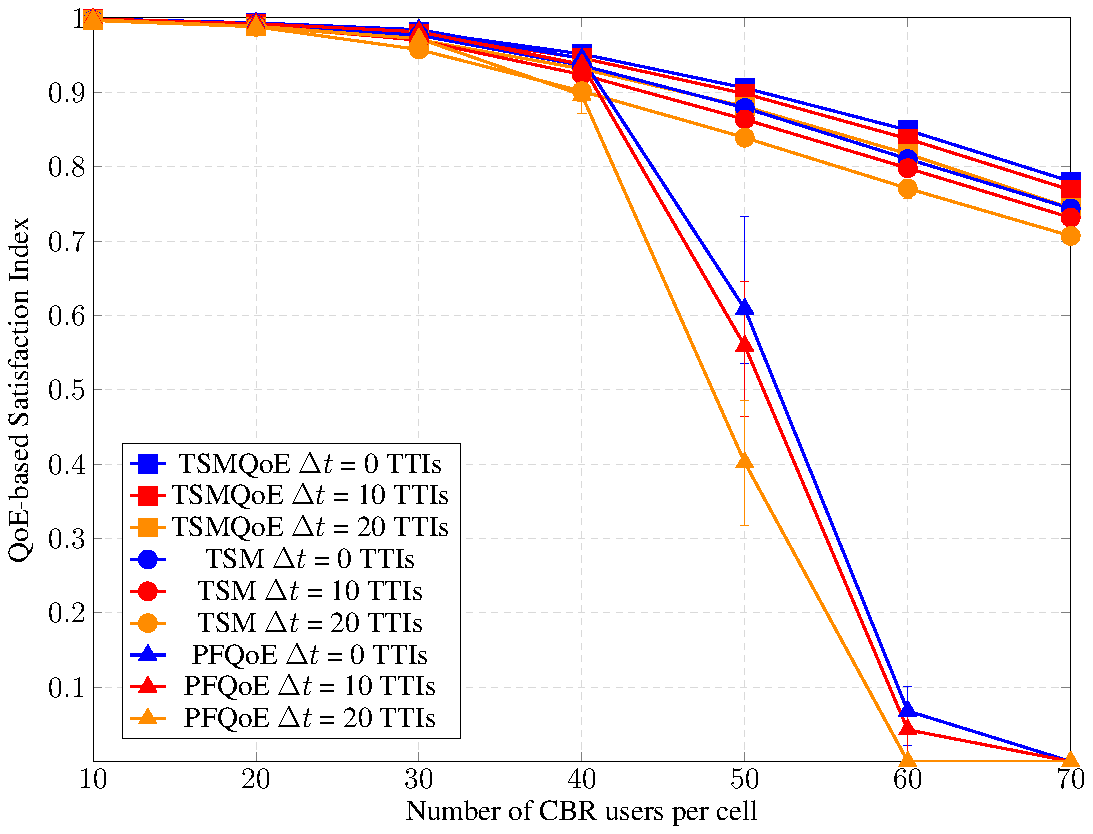
\includegraphics[width=0.55\linewidth,page=1]{figs_wp2/figs_BRUNO_PEDRO/NRT}
	\caption{QoE-based satisfaction index for different algorithms with \ac{CBR} service.}   
	\label{Fig:SatisfactionNRT}
\end{figure}

The fairness during resource allocation for different system loads and algorithms is shown in \FigRef{Fig:FairnessNRT}. The PFQoE algorithm is able to keep the fairness at high values for all system loads, while the fairness index decreases when the system load increases for the TSM and TSMQoE algorithms. The reason for the is that the PFQoE algorithm was designed to guarantee such high fairness values, assuming a trade-off between high user data rates and high fairness values, which decreases its overall satisfaction index. The fairness index for the TSM and TSMQoE techniques tends to follow the trend of the satisfaction index, as it can be seen comparing figures \ref{Fig:SatisfactionNRT} and \ref{Fig:FairnessNRT}. Regarding the CSI degradation, one can see that the fairness values for the PFQoE are not affected by the increase of $\Delta t$, which is expected since its objective is to keep high fairness values independently of the users' channel conditions. The fairness values for the TSM and TSMQoE decreased with the increase of $\Delta t$, as expected.

\begin{figure}[!hb]
	\centering
	\includegraphics[width=0.55\linewidth,page=2]{figs_wp2/figs_BRUNO_PEDRO/NRT}
	\caption{Fairness index for different algorithms with CBR service.}
	\label{Fig:FairnessNRT}
\end{figure}

%The mean cell throughput as a function of the number of CBR users is presented in \FigRef{Fig:CapacityNRT}. For low system loads, the capacity provided by all algorithms is very similar. When the system load increases, we can see that the performance of the TSMQoE algorithm is always slightly higher than that of the TSM algorithm. Moreover, the capacity of these algorithms are lower than the capacity of the PFQoE for low system loads. However, when the system load increases, the capacity of the PFQoE and TSM are very close, and the best capacity is provided by the TSMQoE. The reason for this is the user priority defined by the combination of the weights for the TSMQoE. 

%\begin{figure}[!hb]
%	\centering
%	\includegraphics[width=0.55\linewidth,page=3]{figs_wp2/figs_BRUNO_PEDRO/NRT}
%	\caption{Mean cell throughput for different algorithms with CBR service.}
%	\label{Fig:CapacityNRT}
%\end{figure}

%In \FigRef{Fig:WeightsForTSMQoE}, one can see that the priority function for the TSMQoE presents a heavier right-hand side tail than the priority function for the TSM, which allows assigning resources for users with higher throughput values, increasing the total cell capacity.

\subsubsection{\ac{RT} Service}

In this section, the performance of the proposed DSMQoE technique is compared with the \ac{DSM} algorithm and a QoE-based algorithm called here QoE Scheme. Firstly, the algorithms are evaluated under distinct network errors (see \SecRef{Sec:UtilFramework}), and then, the performance of algorithms are assessed assuming \ac{CSI} imperfections.

%\paragraph{Network Error Analysis\\}
%
%\FigRef{Fig:SatisfactionRTERROR} presents the \ac{QoE}-based satisfaction considering scenarios undergoing different network errors. Regarding \FigRef{Fig:MOSxNetworkError}, the higher network error $\varepsilon$ is, the lower the maximum \ac{MOS}. Thus, we have a satisfaction degradation for all algorithms when the network error value increases because the QoE-based satisfaction is calculated taking into account the user \ac{MOS}, as showed in \SecRef{Sec:SystemModeling}. Therefore, for higher network error values, we obtain lower maximum \ac{MOS} values. In the case of network error equals to 0\%, i.e., no network error, the performance of all algorithms is very similar, with a small disadvantage for the QoE Scheme algorithm. Analyzing the increase of the network error, the DSMQoE presents the best performance for a network error of 2\% because of the combination of the weights employed by this algorithm, which allows users to get a high priority for the resource allocation when their end-to-end delay is at low values (see \FigRef{Fig:WeightsForDSMQoE}), differently from the DSM. Notice that for a network error of 4\% and high system loads, none of the algorithms presents a satisfactory performance.
%
%\begin{figure}[!hbt]
%	\centering
%	\includegraphics[width=0.55\linewidth, page=4]{figs_wp2/figs_BRUNO_PEDRO/plotsCSI}
%	\caption{QoE-based satisfaction index for different algorithms with VoIP service and different percentages of network errors.}   
%	\label{Fig:SatisfactionRTERROR}
%\end{figure}
%
%The fairness index based on the \ac{FER} as a function of the number of \ac{RT} users is depicted in \FigRef{Fig:FairnessRTERROR}. As expected, the \ac{QoE} Scheme provides the  highest levels of fairness due its $\nu$ parameter based on the \ac{PF} algorithm (explained in \SecRef{Sec:stateOfTheArtAlg}), which allows to the QoE Scheme algorithm to also achieve high fairness values as the PF algorithm. This feature results into a unperceived variation of this metric under network error variations. The \ac{DSM} algorithm presents a satisfactory performance in terms of fairness, which is not affected by the increase in the network error because the DSM framework does not take into account the MOS values and the fairness is calculated only based on a QoS metric.  DSMQoE achieved the lowest fairness values because of its low MOS variation for small delay values, which causes the users with low delay values to wait more for the scheduling because they do not achieve high priority values.  
%
%\begin{figure}
%	\centering
%	\includegraphics[width=0.55\linewidth,page=5]{figs_wp2/figs_BRUNO_PEDRO/plotsCSI}
%	\caption{Fairness index for different algorithms with VoIP service and different percentages of network errors.}
%	\label{Fig:FairnessRTERROR}
%\end{figure}
%
%The system capacity is shown in \FigRef{Fig:CapacityRTERROR}. The \ac{DSM} technique outperforms the other algorithms and, as explained before, its performance is not degraded by network error variations due its \ac{QoS} formulation. On the other extreme, the \ac{QoE} Scheme presents the lowest levels of capacity. Notice the there is an intrinsic trade-off between fairness and system capacity, so that the \ac{QoE} Scheme provides the best fairness levels in \FigRef{Fig:FairnessRTERROR} with almost no loss in performance. However in terms of capacity, the QoE Scheme technique experiences the highest performance variations under network errors. \ac{DSM} and DSMQoE algorithms do not present a performance as satisfactory as the \ac{QoE} Scheme in terms of fairness, but they outperform the QoE scheme in terms of system capacity.
%
%\begin{figure}
%	\centering
%	\includegraphics[width=0.55\linewidth,page=6]{figs_wp2/figs_BRUNO_PEDRO/plotsCSI}
%	\caption{Mean cell throughput for different algorithms with VoIP service and different percentages of core network errors.}
%	\label{Fig:CapacityRTERROR}
%\end{figure}

\paragraph{\ac{CSI} analysis}
In this section, we present the simulation results obtained when comparing our proposed algorithm DSMQoE with the \ac{DSM} and \ac{QoE} Scheme techniques under different measurement delays $\Delta t$. We consider for our simulations the network error $\varepsilon$ equal to 2\%.

\FigRef{Fig:SatisfactionRTCSI} presents the \ac{QoE}-based satisfaction for different values of $\Delta t$ for the scenario composed of VoIP users. Note that for all $\Delta t$ variations, the DSMQoE algorithm outperforms the other techniques in terms of satisfaction levels because this algorithm allows users to get higher priority values even for low end-to-end delay values. This occurs due to the weights' multiplication employed by this technique. Analyzing the variations in the $\Delta t$ values, one can see that the DSM technique is more sensitive to CSI imperfections, while the DSMQoE and the QoE Scheme present similar degradation under the $\Delta t$ variations.

\begin{figure}
	\centering
	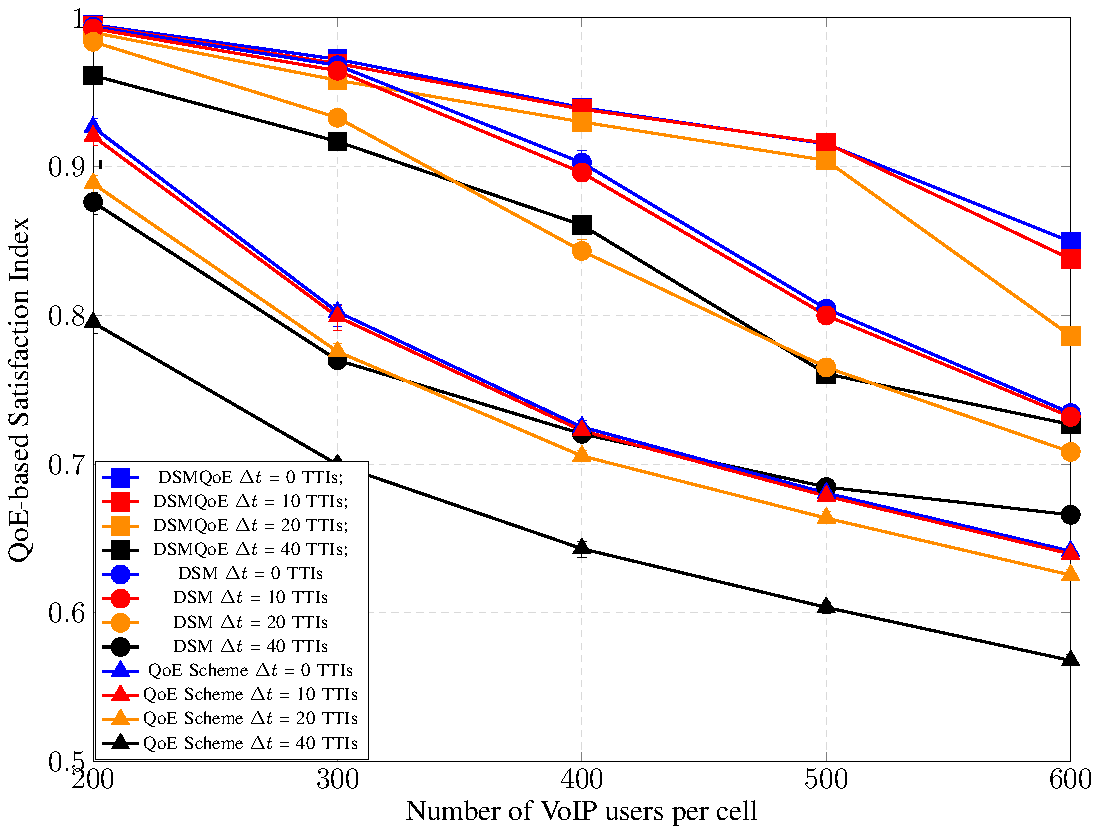
\includegraphics[width=0.55\linewidth,page=1]{figs_wp2/figs_BRUNO_PEDRO/plotsCSI}
	\caption{QoE-based satisfaction index for different algorithms with VoIP service and different CSI time delays.}   
	\label{Fig:SatisfactionRTCSI}
\end{figure}

\FigRef{Fig:FairnessRTCSI} presents the fairness index for different system loads and values of $\Delta t$. As expected, the \ac{QoE} Scheme outperforms the others algorithms and also present the lowest variation with increase of \ac{CSI} measurement delay. This behavior is presented due to $\nu$ parameter in its formulation (as explained in \SecRef{Sec:stateOfTheArtAlg}) and even under high values of delays $\Delta t$, the scheduler keeps a fair resource allocation. The fairness degradation for DSM and DSMQoE is similar, but DSM outperforms DSMQoE due its smoother priority scheduling. On the other hand, the DSMQoE algorithm have an abrupt scheduling due to the MOS function, presenting the lowest fairness values. 

\begin{figure}
	\centering
	\includegraphics[width=0.55\linewidth,page=2]{figs_wp2/figs_BRUNO_PEDRO/plotsCSI}
	\caption{Fairness index for different algorithms with VoIP service and different CSI time delays.}
	\label{Fig:FairnessRTCSI}
\end{figure}

%The mean cell throughput is depicted in \FigRef{Fig:CapacityRTCSI}. The QoE Scheme presents the worst performance in terms of cell capacity due to the trade-off between capacity and fairness. In other words, this technique aims to perform a fair resource allocation, giving many resources to users in bad channel conditions. Thus, high values of total system capacity are not reached and the maximum fairness is obtained as presented in \FigRef{Fig:FairnessRTCSI}. The DSM algorithm achieves capacity levels slightly higher than the DSMQoE scheduler. The QoE Scheme algorithm is very sensitive to $\Delta t$ variations, while the DSM and DSMQoE techniques are not. This happens because in the QoE Scheme formulation it considers the users' channel conditions twice (see \SecRef{Sec:stateOfTheArtAlg}), which results in a higher degradation with the increase of the $\Delta t$ values. 

%\begin{figure}
%	\centering
%	\includegraphics[width=0.55\linewidth,page=3]{figs_wp2/figs_BRUNO_PEDRO/plotsCSI}
%	\caption{Mean cell throughput for different algorithms with VoIP service and different CSI time delays.}
%	\label{Fig:CapacityRTCSI}
%\end{figure}
\section{Conclusion and Perspectives}
\label{Sec:conclusion}
The results presented in \SecRef{Sec:Results} confirms that our objective of proposing efficient \ac{RRA} QoE algorithms, namely TSMQoE and DSMQoE, to improve user satisfaction in a scenario with either NRT or RT services was achieved. Moreover, we present a generalized utility-based QoE/QoS framework suitable for both NRT and RT services that can be used  for different objectives. The reason of this characteristics is that the TSMQoE/DSMQoE techniques use a bell-shaped marginal utility combined with a MOS derivative. Notice that the operator can adopt other utility or mapping functions.
From the system-level simulations results presented in \SecRef{Sec:Results}, it can be concluded that the proposed TSMQoE and DSMQoE techniques outperform the other algorithms in terms of QoE-based satisfaction presenting also satisfactory performance in terms of fairness.

For future work, we can extend this framework to multiple services and multiple antenna schemes in order to further improve the system performance.

%\begin{appendix}
%	\section{Utility-Based Optimization Formulation for Non Real-Time Services}
%	\label{AppendixA}
%	The considered optimization problem for \ac{NRT} services is the maximization of total utility with respect to the users' MOS:
%	%
%	\begin{equation}
%	\label{Eq:UtilOptProbNRTQoE}
%	\underset{\mathcal{K}_j}{\text{max}} \sum_{j=1}^{J} U\left(\Phi\left(T_j[n]\right)\right), 
%	\end{equation}
%	where $U(\Phi(T_j[n]))$ is a utility function where the input parameter is the MOS function $\Phi(T_j[n])$.
%	We consider in this work that the throughput of user $j$ is calculated using an exponential smoothing filtering as indicated below:
%	\begin{equation}
%	\label{Eq:ThroughputCalculationApp}
%	T_{j}\left[n\right] = \left(1 - f_{\mathrm{thru}}\right) \cdot T_{j}\left[n-1\right] + f_{\mathrm{thru}} \cdot \mathcal{R}_j[n],
%	\end{equation}
%	%
%	where $\mathcal{R}_j[n]$ is the instantaneous date rate of user $j$ and $f_{\mathrm{thru}}$ is a filtering constant.
%	
%	Evaluating the objective function in \EqRef{Eq:UtilOptProbNRTQoE} and the throughput expression in \EqRef{Eq:ThroughputCalculationApp}, the derivative of $U(\Phi(T_j[n]))$ with respect to the transmission rate $\mathcal{R}_j$ can be simplified by
%	%
%	\begin{equation}
%	\begin{split}
%	\dfrac{\partial U\left(\Phi\left(T_j\right)\right)}{\partial \mathcal{R}_j} & = \dfrac{\partial U\left(\Phi\left(T_j\right)\right)}{\partial \Phi} \cdot \dfrac{\partial\Phi\left(T_j\right)}{\partial T_j} \cdot \dfrac{\partial T_j}{\partial \mathcal{R}_j} \\ & = \left. \dfrac{\partial U\left(\Phi\left(T_j\right)\right)}{\partial \Phi} \right|_{\Phi = \Phi \left(T_{j}\right)} \cdot \left. \dfrac{\partial\Phi\left(T_j\right)}{\partial T_j} \right|_{T_{j} = \left(1 - f_{\mathrm{thru}}\right) \cdot T_{j}\left[n-1\right] + f_{\mathrm{thru}} \cdot \mathcal{R}_j[n]} \cdot f_{\mathrm{thru}}.
%	\end{split}
%	\end{equation}
%	
%	In the case that $f_{\mathrm{thru}}$ is sufficiently small, the expression above can be simplified as follows \cite{Art:Song2005_p2}:
%	%
%	\begin{equation}
%	\label{Utility_Derivative_NRT_QoE_2}
%	\dfrac{\partial U\left(\Phi\left(T_j\right)\right)}{\partial \mathcal{R}_j} \approx  \left. \dfrac{\partial U\left(\Phi\left(T_j\right)\right)}{\partial \Phi} \right|_{\Phi = \Phi \left(T_{j}\right)} \cdot \left. \dfrac{\partial\Phi\left(T_j\right)}{\partial T_j} \right|_{T_{j} = T_{j}\left[n-1\right]} \cdot f_{\mathrm{thru}},
%	\end{equation}
%	%
%	where the previous resource allocation totally determines the current values of the marginal utilities. Using the one-order Taylor formula \cite{Art:Song2005_p2, Phd:Emanuel2011} and considering \eqref{Utility_Derivative_NRT_QoE_2}, we have
%	%
%	\begin{equation}\label{Eq:Taylor_NRT_QoE1}
%	\begin{split}
%	&\sum_{j=1}^{J} U\left(\Phi\left(T_j\left[n\right]\right)\right) \approx \sum_{j=1}^{J} U\left(\Phi\left(T_j\left[n-1\right]\right)\right) + \\
%	&\left(T_{j}\left[n\right]-T_{j}\left[n-1\right]\right) \cdot \sum_{j=1}^{J} \left. \dfrac{\partial U\left(\Phi\left(T_j\right)\right)}{\partial \Phi}  \right|_{\Phi = \Phi \left(T_{j}[n - 1]\right)} \cdot \left. \dfrac{\partial \Phi\left(T_j\right)}{\partial T_j} \right|_{T_{j} = T_{j}[n - 1]},
%	\end{split}
%	\end{equation} 
%	% 
%	from the throughput expression given in \EqRef{Eq:ThroughputCalculationApp}, we have that
%	%
%	\begin{equation}
%	\begin{split}
%	T_j[n] &= (1-f_{\mathrm{thru}}) \cdot T_j[n-1]+f_{\mathrm{thru}} \cdot \mathcal{R}_j[n]
%	\\
%	T_j[n] &= T_j[n-1]- f_{\mathrm{thru}} \cdot T_j[n-1] + \mathcal{R}_j[n]
%	\\
%	T_j[n]- T_j[n-1] &= f_{\mathrm{thru}} \cdot \mathcal{R}_j[n]- f_{\mathrm{thru}} \cdot T_j[n-1],
%	\end{split}
%	\end{equation}
%	%
%	thus, the expression \EqRef{Eq:Taylor_NRT_QoE1} becomes
%	%
%	\begin{equation}\label{Eq:Taylor_NRT_QoE}
%	\begin{split}
%	&\sum_{j=1}^{J} U\left(\Phi\left(T_j[n]\right)\right) \approx \sum_{j=1}^{J} U\left(\Phi\left(T_j[n-1]\right)\right) + \\ &\left(f_{\mathrm{thru}} \cdot \mathcal{R}_j[n] - f_{\mathrm{thru}} \cdot T_j[n-1]\right) \cdot \sum_{j=1}^{J} \left. \dfrac{\partial U\left(\Phi\left(T_j\right)\right)}{\partial \Phi} \right|_{\Phi = \Phi \left(T_{j}[n - 1]\right)}   \cdot \left. \dfrac{\partial \Phi\left(T_j\right)}{\partial T_j} \right|_{T_{j} = T_{j}[n - 1]}.
%	\end{split}
%	\end{equation}
%	
%	Let us consider the maximization of \eqref{Eq:Taylor_NRT_QoE}. Notice that the maximization of the left side of expression \eqref{Eq:Taylor_NRT_QoE} is our original optimization problem given by \eqref{Eq:UtilOptProbNRTQoE}. The maximization of the right side of expression \eqref{Eq:Taylor_NRT_QoE} is the new simplified optimization problem. Since $f_{\mathrm{thru}}$ is a constant and $T_j\left[n-1\right]$ is known and fixed before the resource allocation at the current \ac{TTI} $n$, the new simplified optimization problem becomes linear in terms of the instantaneous user's data rate, and is given by
%	%
%	\begin{equation}
%	\label{Eq:Simple_Obj_Function_NRT_QoE_App}
%	\underset{\mathcal{K}_j}{\text{max}} \sum_{j=1}^{J} U^{'}\left(\Phi\left(T_j[n-1]\right)\right) \cdot \Phi^{'}\left(T_j[n-1]\right) \cdot \mathcal{R}_j[n].
%	\end{equation}
%	
%	Notice that we started with an optimization formulation based on throughput given by \eqref{Eq:UtilOptProbNRTQoE}, made some logical assumptions and mathematical simplifications, and ended up with a linear optimization formulation based on instantaneous rates given by \eqref{Eq:Simple_Obj_Function_NRT_QoE_App}. According to these arguments, we claim that the instantaneous optimization maximizing \eqref{Eq:Simple_Obj_Function_NRT_QoE_App} leads to a long-term optimization that maximizes \eqref{Eq:UtilOptProbNRTQoE}.
%	
%	For  \ac{NRT} services, $\dfrac{\partial U\left(\Phi\left(T_j[n]\right)\right)}{\partial \Phi}$ can be calculated by:
%	%
%	\begin{equation}
%	\begin{split}
%	\dfrac{\partial U\left(\Phi\left(T_j[n]\right)\right)}{\partial \Phi} &= \dfrac{\partial }{\partial \Phi}  \left(\dfrac{1}{\left(1+e^{\mu \cdot \sigma \cdot(\Phi(T_j[n])-\Phi^\mathrm{req})}\right)^2}\right)\\
%	&= \dfrac{- \mu  e^{\mu (\Phi(T_j[n]) - \Phi^{\text{req}}) / \sigma}}{\sigma \left(1 + e^{\mu (\Phi(T_j[n]) - \Phi^{\text{req}}) / \sigma}\right)^{2}}.
%	\end{split}
%	\end{equation}	
%	
%	The considered MOS function $\Phi\left(T_j[n]\right)$ was proposed in \cite{Poncela2014} and its expression is
%	%
%	\begin{equation}\label{MOS_FUNC}
%	\Phi\left(T_j[n]\right)= 5 - \frac{578}{1+\left(\dfrac{T_j[n] + 541.1}{45.98}\right)^{2}}.	
%	\end{equation}
%	
%	Thus, $\dfrac{\partial \Phi\left(T_j[n]\right)}{\partial T_{j}}$ can be calculated by:
%	%
%	\begin{equation}
%	\begin{split}
%	\dfrac{\partial \Phi\left(T_j[n]\right)}{\partial T_{j}} &= \dfrac{\partial }{\partial T_j}\left(5 - \frac{578}{1+\left(\dfrac{T_j[n] + 541.1}{45.98}\right)^{2}}\right) = - \dfrac{\partial }{\partial T_j} \left( \frac{578}{1+\left(\dfrac{T_j[n] + 541.1}{45.98}\right)^{2}}\right)\\
%	\\&=\frac{578+\dfrac{\partial }{\partial T_j} \left(1+\left(\dfrac{T_j[n] + 541.1}{45.98}\right)^{2}\right)}{\left[1+\left(\dfrac{T_j[n] + 541.1}{45.98}\right)^{2}\right]^{2}} = \frac{578 \cdot 2 \cdot (T_j[n]+541.1)}{45.98^{2} \cdot\left[1+\left(\dfrac{T_j[n] + 541.1}{45.98}\right)^{2}\right]^{2}}\\
%	\\
%	&= \frac{0.5468 \cdot (T_j[n]+541.1)}{\left[1+\left(\dfrac{T_j[n] + 541.1}{45.98}\right)^{2}\right]^{2}}.
%	\end{split}
%	\end{equation}
%	
%	\clearpage
%	\section{Utility-Based Optimization Formulation for Real-Time Services}
%	\label{AppendixB}
%	As explained in \SecRef{Sec:FormRT}, the utility-based optimization problem in a scenario with \ac{RT} service is the maximization of total utility with respect to the users' MOS and is formulated as:
%	%
%	\begin{equation}
%	\label{Eq:UtilOptProbRT}
%	\underset{\mathcal{K}_j}{\text{max}} \sum_{j=1}^{J} U\left(\Phi\left(R\left(d_j[n]\right)\right)\right), 
%	\end{equation}
%	%
%	where $U\left(\Phi\left(R\left(d_j[n]\right)\right)\right)$ is a utility function where the input parameter is the MOS function $\Phi\left(R\left(d_j[n]\right)\right)$, $R\left(d_j[n]\right)$ is the R factor (which is the primary output of the ITU-T E-model G.107 calculations \cite{itu2005107}) that depends on the end-to-end delay $d_j[n]$.
%	
%	The end-to-end packet delay is calculated by the sum of the \ac{HOL} packet delay imposed by the radio access network ($d_j ^{\text hol}$) and the packet delay imposed by the Core Network ($d_j^{\text core}$):
%	%
%	\begin{equation}
%	\label{Eq:endToEndDelay_App}
%	d_j[n] = d_{j}^\text{hol}[n] + d_j^\text{core}[n].
%	\end{equation}
%	
%	We use a recursive model to calculate the \ac{HOL} packet delay as follows \cite{Rodrigues2014_Wiley}:
%	%
%	\begin{equation}
%	\label{Eq:HOL_Delay_App}
%	d_{j}^\mathrm{hol}\left[n+1\right] = d_{j}^\mathrm{hol}\left[n\right] + t_{\text{tti}} - \frac{1}{L} \cdot \left( \frac{\mathcal{R}_{j}[n] \cdot t_{\text{tti}}}{S_\mathrm{p}}\right),
%	\end{equation}
%	%
%	where $t_{\text{tti}}$ is the duration of the \ac{TTI} in seconds, $L$ is the packet arrival rate, $S_\mathrm{p}$ is the packet size, and $\mathcal{R}_{j}[n]$ is the instantaneous achievable transmission rate on \ac{TTI} $n$.
%	
%	Evaluating the objective function in \EqRef{Eq:UtilOptProbRT}, the derivative of $U\left(\Phi\left(R\left(d_j\right)\right)\right)$ with respect to the transmission rate $\mathcal{R}_j$ is given by			
%	\begin{equation}
%	\begin{split}
%	\dfrac{\partial U\left(\Phi\left(R\left(d_j\right)\right)\right)}{\partial \mathcal{R}_j} &= \dfrac{\partial U\left(\Phi\left(R\left(d_j\right)\right)\right)}{\partial \Phi} \cdot  \dfrac{\partial \Phi\left(R\left(d_j\right)\right)}{\partial d_j} \cdot \dfrac{\partial d_{j}}{\partial \mathcal{R}_j} \\ &= \dfrac{\partial U\left(\Phi\left(R\left(d_j\right)\right)\right)}{\partial \Phi} \cdot  \dfrac{\partial \Phi\left(R\left(d_j\right)\right)}{\partial d_j} \cdot \left(-\frac{t_{\mathrm{tti}}}{L \cdot S_\mathrm{p}} \right).
%	\end{split}
%	\end{equation}
%	
%	Using the result above and assuming that the \ac{TTI} duration is sufficiently small, the Lagrange theorem of the mean can be used \cite{Proc:Lei2007,Phd:Emanuel2011}, which says that 
%	%
%	\begin{equation}\label{Eq:Mean_Theorem_RT_QoE}
%	\begin{split}
%	&\sum_{j=1}^{J} U\left(\Phi\left(R\left(d_j[n+1]\right)\right)\right) \approx \\ & \sum_{j=1}^{J} U\left(\Phi\left(R\left(d_j[n]\right)\right)\right) + \left.\sum_{j=1}^{J} \dfrac{\partial U\left(\Phi\left(R\left(d_j\right)\right)\right)}{\partial \mathcal{R}_j}\right\vert_{\mathcal{R}_j=\mathcal{R}_j[n-1]} \cdot \left( \mathcal{R}_j[n] - \mathcal{R}_j\left[n-1\right]\right) = \\
%	& \sum_{j=1}^{J} U\left(\Phi\left(R\left(d_j[n]\right)\right)\right) + \left. \sum_{j=1}^{J} - \dfrac{\partial U\left(\Phi\left(R\left(d_j\right)\right)\right)}{\partial \Phi}\right\vert_{\Phi=\Phi\left(R\left(d_j\right)\right)}  \cdot  \left.\dfrac{\partial \Phi\left(R\left(d_j\right)\right)}{\partial d_j}\right\vert_{d_j=d_j[n-1]} \cdot \\ &\frac{t_{\mathrm{tti}}}{L \cdot S_\mathrm{p}} \cdot \left( \mathcal{R}_j[n] - \mathcal{R}_j\left[n-1\right]\right) = \\
%	& \sum_{j=1}^{J} U\left(\Phi\left(R\left(d_j[n]\right)\right)\right) + \left. \sum_{j=1}^{J} \dfrac{\partial U\left(\Phi\left(R\left(d_j\right)\right)\right)}{\partial \Phi}\right\vert_{\Phi=\Phi\left(R\left(d_j\right)\right)}  \cdot  \left.\left|\dfrac{\partial \Phi\left(R\left(d_j\right)\right)}{\partial d_j}\right|\right\vert_{d_j=d_j[n-1]} \cdot \\ &\frac{t_{\mathrm{tti}}}{L \cdot S_\mathrm{p}} \cdot \left( \mathcal{R}_j[n] - \mathcal{R}_j\left[n-1\right]\right).
%	\end{split}
%	\end{equation}
%	
%	The absolute value operator is used in \eqref{Eq:Mean_Theorem_RT_QoE} because the MOS function $\Phi\left(R\left(d_j\right)\right)$ is assumed to be decreasing, which yields negative marginal utilities and cancels the negative sign in \eqref{Eq:Mean_Theorem_RT_QoE}.
%	
%	On one hand, the maximization of the left side of expression \eqref{Eq:Mean_Theorem_RT_QoE} is our original optimization problem given by \eqref{Eq:UtilOptProbRT}. On the other hand, the maximization of the right side of expression \eqref{Eq:Mean_Theorem_RT_QoE} is the new simplified optimization problem. We have that $t_{\mathrm{tti}}$, $L$ and $S_\mathrm{p}$ are constants, and that $d_{j}^{\mathrm{hol}}\left[n\right]$ and $\mathcal{R}_j\left[n-1\right]$ are known and fixed before the resource allocation at \ac{TTI} $n$. Therefore, the new simplified optimization problem becomes linear in terms of the instantaneous user's data rate, and is given by
%	
%	\begin{equation}
%	\label{Eq:ModProblem}
%	\underset{\mathcal{K}_j}{\text{max}} \sum_{j=1}^{J} U^{'}\left(\Phi\left(R\left(d_j[n]\right)\right)\right) \cdot  \Phi^{'}\left(R\left(d_j[n]\right)\right) \cdot \mathcal{R}_j[n].
%	\end{equation}
%	
%	%\begin{equation}
%	%\label{Eq:ModProblem}
%	%\underset{\mathcal{K}_j}{\text{max}} \sum_{j=1}^{J} \left. \dfrac{\partial U(\Phi(R(d_j[n])))}{\partial \Phi}\right\vert_{\Phi = \Phi(R(d_{j}[n - 1]))} \cdot \left. \dfrac{\partial \Phi(R(d_j[n]))}{\partial {d_j}} \right\vert_{d_{j} = d_{j}[n - 1]}\cdot \mathcal{R}_j[n].
%	%\end{equation}
%	
%	For  \ac{RT} services, $\dfrac{\partial U\left(\Phi\left(R\left(d_j[n]\right)\right)\right)}{\partial \Phi}$ can be calculated by:
%	%
%	\begin{equation}
%	\begin{split}
%	\dfrac{\partial U\left(\Phi\left(R\left(d_j[n]\right)\right)\right)}{\partial \Phi} &= \dfrac{\partial }{\partial \Phi}  \left(\dfrac{1}{\left(1+e^{\mu \cdot \sigma \cdot \left(\Phi\left(R(d_j[n])\right)-\Phi^\mathrm{req}\right)}\right)^2}\right)\\
%	&= \dfrac{- \mu  e^{\mu \left(\Phi\left(R\left(d_j[n]\right)\right) - \Phi^{\text{req}}\right) / \sigma}}{\sigma \left(1 + e^{\mu \left(\Phi\left(R\left(d_j[n]\right)\right) - \Phi^{\text{req}}\right) / \sigma}\right)^{2}}.
%	\end{split}
%	\end{equation}	
%	
%	Evaluating the MOS expression in \SecRef{Sec:FormRT} (\EqRef{MOS_DELAY_FUNC}), its derivative is given by:
%	
%	\begin{equation}
%	\Phi^{'}\left(R\left(d_j[n]\right)\right) = \dfrac{\partial \Phi\left(R\left(d_j[n]\right)\right)}{\partial R} \cdot \dfrac{\partial R\left(d_j[n]\right)}{\partial d_j}, 
%	\end{equation}
%	
%	Then, we have that
%	%
%	{\small\begin{equation}
%		\label{Eq:dMOSDR}
%		\begin{split}
%		\dfrac{\partial \Phi\left(R\left(d_j\right)\right)}{\partial R} = &\dfrac{\partial}{\partial R} \left(1+ 0.035\cdot R\left(d_j\right)+ R\left(d_j\right) \cdot \left(R\left(d_j\right) - 	60\right) \cdot \left(100 - R\left(d_j\right)\right)\cdot 7 \cdot  10^{-6}\right)\\ = &\dfrac{\partial  }{\partial R}\left(1 + 0.035R\left(d_j\right) + \left(R^{2}\left(d_j\right) - 60R\left(d_j\right)\right)\left(100 - R\left(d_j\right)\right)\cdot 7 \cdot  10^{-6}\right) \\ =
%		&\dfrac{\partial}{\partial R}\left(1 + 0.035R\left(d_j\right) + \left(100R^{2}\left(d_j\right) + 60R^{2}\left(d_j\right)\right) \cdot 7 \cdot  10^{-6}\right) \\ =
%		&\dfrac{\partial }{\partial R}\left(1 + 0.035R\left(d_j\right) + 160R^{2}\left(d_j\right)\cdot 7 \cdot  10^{-6}\right) \\ = &0.035 + 320 \cdot 7 \cdot  10^{-6}R\left(d_j\right),
%		\end{split}
%		\end{equation}}
%	%
%	and,
%	%
%	{\footnotesize\begin{equation}
%		\label{dRdDelay}
%		\begin{split}
%		\dfrac{\partial R\left(d_j\right)}{\partial d_j} = & \dfrac{\partial}{\partial d_j} \left(94.2+ 0.024\cdot d_j -  0.11 \cdot \left(d_j - 177.3\right) \cdot H\left(d_j - 177.3\right)-11 - 40ln\left(1 + 10\varepsilon\right)+10 \right) \\ = &\dfrac{\partial}{\partial d_j}\left(94.2 - 0.024d_j - \left(0.11d_j - 19.503\right)\cdot \left(H\left(d_j - 177.3\right)\right)- 11- 40ln\left(1 + 10\varepsilon \right)+10\right)\\ = &- 0.024 - 0.11\cdot H\left(d_j - 177.3\right) - D\left(d_j - 177.3\right)\left(0.11d_j - 19.503\right),
%		\end{split}
%		\end{equation}}
%	%
%	where $H(x)$ is the unit step function, $D(x)$ is the unitary impulse function.
%	
%\end{appendix}

%%End of APPENDIX

%\begin{thebibliography}{00}
%\bibitem{b1} G. Eason, B. Noble, and I. N. Sneddon, ``On certain integrals of Lipschitz-Hankel type involving products of Bessel functions,'' Phil. Trans. Roy. Soc. London, vol. A247, pp. 529--551, April 1955.
%\bibitem{b2} J. Clerk Maxwell, A Treatise on Electricity and Magnetism, 3rd ed., vol. 2. Oxford: Clarendon, 1892, pp.68--73.
%\bibitem{b3} I. S. Jacobs and C. P. Bean, ``Fine particles, thin films and exchange anisotropy,'' in Magnetism, vol. III, G. T. Rado and H. Suhl, Eds. New York: Academic, 1963, pp. 271--350.
%\bibitem{b4} K. Elissa, ``Title of paper if known,'' unpublished.
%\bibitem{b5} R. Nicole, ``Title of paper with only first word capitalized,'' J. Name Stand. Abbrev., in press.
%\bibitem{b6} Y. Yorozu, M. Hirano, K. Oka, and Y. Tagawa, ``Electron spectroscopy studies on magneto-optical media and plastic substrate interface,'' IEEE Transl. J. Magn. Japan, vol. 2, pp. 740--741, August 1987 [Digests 9th Annual Conf. Magnetics Japan, p. 301, 1982].
%\bibitem{b7} M. Young, The Technical Writer's Handbook. Mill Valley, CA: University Science, 1989.
%\end{thebibliography}
\bibliographystyle{IEEEtran}
%\bibliography{ufc40}
%\bibliographystyle{IEEEtran}
\bibliography{IEEEabrv,IEEEexample}

\end{document}
